\chapter{Aplikacja}
\section{Program prezentacji danych}
Aplikacja została wykonana z myślą o pracodawcy, który chciałby mieć podgląd obecnych pracowników w biurze, oraz podsumowanie przepracowanego czasu dla poszczególnego pracownika.
\subsection{Podgląd obecnych pracowników}
W tej części programu można podejżeć obecnych pracowników ich imię, nazwisko oraz czas przybycia.
Widok odświeża się do pół sekundy.
\begin{figure}[h!]
	\centering
	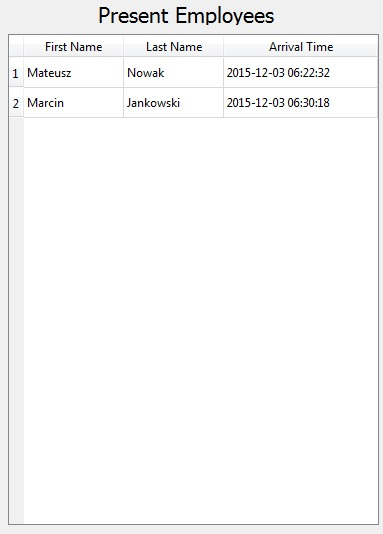
\includegraphics[]{img/present_employees.jpg}
	\label{fig:present_employees}
	\caption[Obecni pracownicy]{Obecni pracownicy}
\end{figure}
\subsection{Podgląd prepracowanego czasu pracowników}
Podgląd umożliwia wybrania przedziału czasu. Nastepnie wyświetli się imie, nazwisko oraz przepracowany czas.
\begin{figure}[h!]
	\centering
	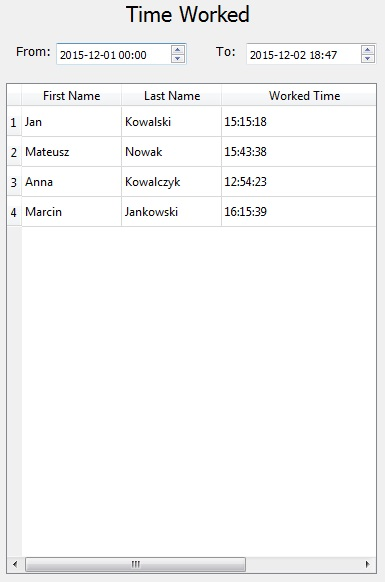
\includegraphics[]{img/time_worked.jpg}
	\label{fig:time_worked}
	\caption[Przepracowany czas]{Przepracowany czas}
\end{figure}
\newpage
\subsection{Dodawanie pracowników}
Ta część programu pozwala na dodawanie użytkowników. Wymagane są wszystkie pola do wpsiania.
Należy podać: Imię, Nazwisko, id taga rfid. email oraz hasło do systemu.
\begin{figure}[h!]
	\centering
	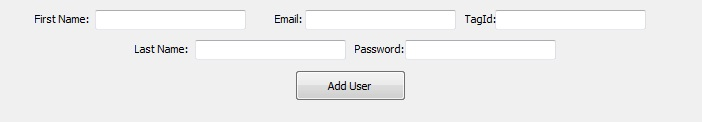
\includegraphics[]{img/add_user.jpg}
	\label{fig:add_user}
	\caption[Dodaj pracownika]{Dodaj pracownika}
\end{figure}
\section{Technologie}
Wykorzystane technologie:
\begin{itemize}
\item Python3.4 - Język programowania, w którym została wykonana aplikacja.
\item PyQt5 - Biblioteka języka python do interfejsu graficznego.
\item psycopg2 - Biblioteka języka python do komunikacji z bazą danych PostgreSQL
\item PostgreSQL - Baza danych.
\item Vagrant - Środowisko do przygotowania maszyn wirtualnych.
\item Raspbian - Dystrybujca linuxa przygotowanego dla RPi na podstawie dystrybucji Debian.
\end{itemize}
\section{Przygotowanie środowiska}
Aby uruchomić program prezentacji danych potrzeba zainstalować interpreter Python3.4, oraz biblioteki PyQt5, psycopq2. Program używa danych przetrzymywanych w bazie danych PostgreSQL.
\section{Baza Danych}
Baza danych składa się z dwóch tabel, Pracowników oraz przejść. Do każdego pracownika może być przypisane wiele przejść.

\begin{figure}[h!]
	\centering
	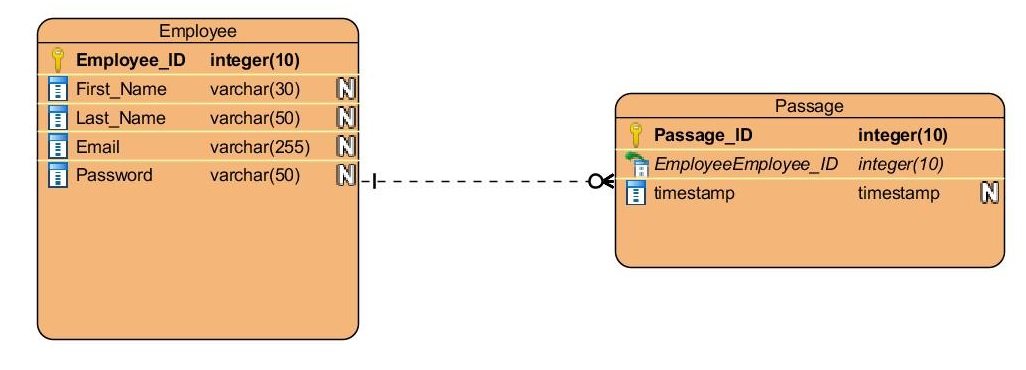
\includegraphics[width=\linewidth]{img/ERD_screen.jpg}
	\label{fig:ERD}
	\caption[Diagram ERD]{Diagram ERD}
\end{figure}
Możliwe jest ustawinie bazy danych na dowolonym urządzeniu. Takie rozwiązanie było niezbedne ze względu na to, że posiadaliśmy tylko jeden komputer RPi. Aplikacja prezentacji danych, komunikuje się wyłącznie z bazą danych, więc możliwe było tworzenie aplikacji bez komputera RPi.
\subsection{Baza danych na maszynie wirtualnej}
W ramach projektu został przygotowany plik konfiguracyjny maszyny\\ (github:/database/Vagrantfile). Aby wygenerować maszynę wirtualną potrzebny jest program Vagrant. Uruchomienie skonfigurowanej maszyny wirtualenej, polega na wejściu do katalogu z plikiem konfigurayjnym i wywołaniem komędy "vagrant up". Następnie trzeba przekazać port 5432 bazy danych z maszyny wirtualnej do systemu operacyjnnego na ip 127.0.0.1, w projekcie wykorzystywany był do tego program putty.
Dane logowania do maszyny wirtualnej to: użytkownik - vagrant, hasło - vagrant.
\subsection{Baza dnych na Raspberry Pi}
Do pracy na RPi Wybraliśmy dystrybucje linuxa Raspbian.
Aby skonfigurować bazę danych na Raspberry Pi należy wykonać następujące komendy:
\lstset{language=bash, breaklines=true}
\begin{lstlisting}
apt-get update
apt-get install postgresql postgresql-contrib postgis gpsbabel git libsqlite3-dev libreadline-dev libpq-dev libbz2-dev zlib1g-dev libpqxx-dev libzip-dev -y
echo -ne "alamakota\nalamakota" | su - postgres -c 'createuser -P -e wbudowane'
su - postgres -c 'createdb -e -O wbudowane wbudowane'
su - postgres -c 'psql wbudowane < /vagrant/czaspracyBD.sql'
su - postgres -c 'psql wbudowane -c "GRANT ALL ON TABLE Employee TO wbudowane;"'
su - postgres -c 'psql wbudowane -c "GRANT ALL ON TABLE Passage TO wbudowane;"'
su - postgres -c 'psql wbudowane -c "GRANT USAGE, SELECT ON ALL SEQUENCES IN SCHEMA public to wbudowane;"'
\end{lstlisting}



